%----------------------------------------------------------------------------------------
%	PACKAGES AND THEMES
%----------------------------------------------------------------------------------------

\documentclass{beamer}

\mode<presentation> {

% The Beamer class comes with a number of default slide themes
% which change the colors and layouts of slides. Below this is a list
% of all the themes, uncomment each in turn to see what they look like.

%\usetheme{default}
%\usetheme{AnnArbor}
%\usetheme{Antibes}
%\usetheme{Bergen}
%\usetheme{Berkeley}
%\usetheme{Berlin}
%\usetheme{Boadilla}
%\usetheme{CambridgeUS}
%\usetheme{Copenhagen}
%\usetheme{Darmstadt}
%\usetheme{Dresden}
%\usetheme{Frankfurt}
%\usetheme{Goettingen}
%\usetheme{Hannover}
%\usetheme{Ilmenau}
%\usetheme{JuanLesPins}
%\usetheme{Luebeck}
\usetheme{Madrid}
%\usetheme{Malmoe}
%\usetheme{Marburg}
%\usetheme{Montpellier}
%\usetheme{PaloAlto}
%\usetheme{Pittsburgh}
%\usetheme{Rochester}
%\usetheme{Singapore}
%\usetheme{Szeged}
%\usetheme{Warsaw}

% As well as themes, the Beamer class has a number of color themes
% for any slide theme. Uncomment each of these in turn to see how it
% changes the colors of your current slide theme.

%\usecolortheme{albatross}
%\usecolortheme{beaver}
%\usecolortheme{beetle}
%\usecolortheme{crane}
%\usecolortheme{dolphin}
%\usecolortheme{dove}
%\usecolortheme{fly}
%\usecolortheme{lily}
%\usecolortheme{orchid}
%\usecolortheme{rose}
%\usecolortheme{seagull}
%\usecolortheme{seahorse}
%\usecolortheme{whale}
%\usecolortheme{wolverine}

%\setbeamertemplate{footline} % To remove the footer line in all slides uncomment this line
%\setbeamertemplate{footline}[page number] % To replace the footer line in all slides with a simple slide count uncomment this line

%\setbeamertemplate{navigation symbols}{} % To remove the navigation symbols from the bottom of all slides uncomment this line
}

\usepackage{graphicx} % Allows including images
\usepackage{booktabs} % Allows the use of \toprule, \midrule and \bottomrule in tables
\usepackage[utf8]{inputenc}
\usepackage{adjustbox}
\usepackage{tikz}
\usetikzlibrary{arrows.meta}
\tikzset{%
  >={Latex[width=2mm,length=2mm]},
  % Specifications for style of nodes:
            base/.style = {rectangle, rounded corners, draw=black,
                           minimum width=4cm, minimum height=1cm,
                           text centered, font=\sffamily},
  activityStarts/.style = {base, fill=blue!30},
       startstop/.style = {base, fill=red!30},
    activityRuns/.style = {base, fill=green!30},
         process/.style = {base, minimum width=2.5cm, fill=orange!15,
                           font=\ttfamily},
}
%----------------------------------------------------------------------------------------
%	TITLE PAGE
%----------------------------------------------------------------------------------------
\title[Viculum]{"VICULUM" \\ Ein virtueller Rundgang durch die Veranstaltungen eines Hochschul-Curriculums } % The short title appears at the bottom of every slide, the full title is only on the title page

\author{Altenberg, Dürr, Milazzo, Röhrle}
\institute[]
{
Hochschule Albstadt-Sigmaringen \\ % Your institution for the title page
\medskip
\textit{Fabian Altenberg (WIN), altenbfa@hs-albsig.de} % Your email address
\newline
\textit{Maik Dürr (TI), duerrmai@hs-albsig.de} % Your email address
\newline
\textit{Domenico Milazzo (TI), milazzdo@hs-albsig.de} % Your email address
\newline
\textit{Prof. Dr. Jörg Röhrle, roehrle@hs-albsig.de} % Your email address
\newline
}
\date{\today} % Date, can be changed to a custom date

\begin{document}

\begin{frame}
\titlepage % Print the title page as the first slide
\end{frame}

\begin{frame}
\frametitle{Überblick}
\begin{enumerate}
\item Die Idee : Konzept und Realisierung eines virtuellen Rundgangs durch die Veranstaltungen eines Modulhandbuchs 
\item Das Konzept: Ein Datenmodell zur vollständigen Erfassung eines Curriculums 
\item Die Realisierung - Datenbankzugriff, Virtualisierung, Implementierung der Kommunikationsschicht
\item Zusammenfassung/Kritik/Ausblick
\end{enumerate}
\end{frame}

%----------------------------------------------------------------------------------------
%	PRESENTATION SLIDES
%----------------------------------------------------------------------------------------

\begin{frame}
\frametitle{Die Idee}
\textbf{Grundgedanke}
\begin{itemize}
\item Implementierung eines natürlichen ("spielerischen") Zugangs zu Studieninhalten, quasi gleichsam als Ersatz der zwar korrekten, jedoch "trockenen" Lektüre des Modulhandbuchs ("Curriculums")
\item Projektion eines Studienverlaufs auf ein mehrstöckiges Gebäude, dessen Etagen die einzelnen Studiensemester und deren Räume wiederum die darin angebotenen Veranstaltungen repräsentieren 
\item Recherchen ergaben:  Bis dato keine vergleichbaren Realisierungen unserer Mitbewerber!
\end{itemize}
\end{frame}

%------------------------------------------------

\begin{frame}
\frametitle{Die Idee}
\textbf{Pflichtenheft}
\begin{itemize}
\item Datenbankgestützte Erfassung des vollständigen Modulhandbuchs zur Bewirtschaftung aller beteiligten Ressourcen 
\item Dynamische Erzeugung von "Szenen", i.e. Veranstaltungen, Studiensemestern ("Etagen"), sowie deren Inhalte und  Zusammenhänge als virtuelle Räumlichkeiten 
\item Zusätzlich Möglichkeit zur Darstellung "repräsentativer" inhaltlicher Auszüge einzelner Veranstaltungen durch Bilder, Tafelaufschriebe oder Videos
\end{itemize}
\end{frame}


%------------------------------------------------

\begin{frame}
\frametitle{Das Konzept - Auswahl der Realisierungsmedien}
\begin{itemize}
\item Serverdatenbanksystem \textbf{ORACLE} als Speichermedium
\item \textbf{"Unity"} zur virtuellen Darstellung von Räumen, Inhalten und Querverweisen 
\item \textbf{C\#} zur Implementierung der Controllerschicht zwischen Datenbank und Virtualisierungssoftware
\end{itemize}
\end{frame}


%------------------------------------------------

\begin{frame}
\frametitle{Das Konzept - Datenbankmodell zur Bewirtschaftung eines Hochschul-Curriculums}
\begin{center}

\includegraphics[width=0.8\textwidth]{pictures/Datenmodell_Viculum.png}
\end{center}
\end{frame}


%------------------------------------------------

\begin{frame}
\frametitle{Das Konzept - Schema der dynamischen Erzeugung von virtualisierten Inhalten}
\begin{adjustbox}{totalheight=\textheight-5\baselineskip}
\begin{columns}[c] % The "c" option specifies centered vertical alignment while the "t" option is used for top vertical alignment

\column{.5\textwidth} % Left column and width

\textbf{Ablauf}
\begin{enumerate}
\item Start einer "Szene" -  Erzeugung eines generischen Unity - Raumobjektes
\item Instanziierung des Raumobjektes und dadurch Schaffung einer konkreten Veranstaltungsszene durch dynamischen Datenbankzugriff via C\#
\item  Anzeige der konkreten Raumszene mit den Inhalten einer Veranstaltung, ihren Abhängigkeiten innerhalb des Curriculums sowie repräsentativen Darstellungen durch Bilder, Texte und/oder Videos
\end{enumerate}

\column{.3\textwidth} % Right column and width
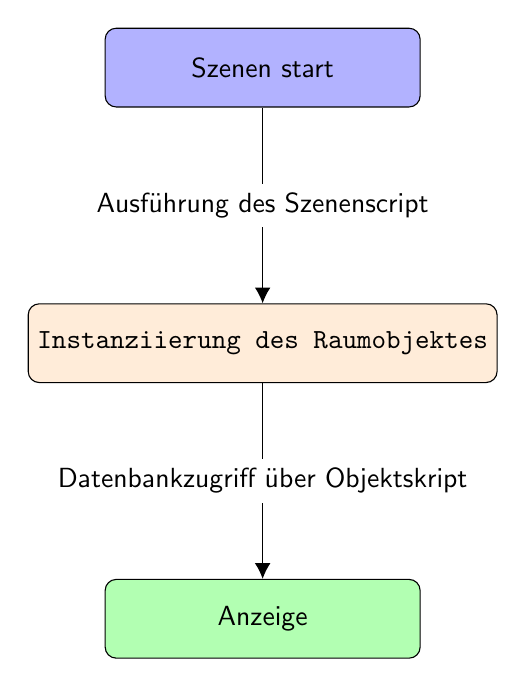
\begin{tikzpicture}[node distance=3.5cm,
    every node/.style={fill=white, font=\sffamily}, align=center]
  % Specification of nodes (position, etc.)
  \node (start)             [activityStarts]              	{Szenen start};
  \node (Object)     [process, below of=start]  {Instanziierung des Raumobjektes};
  \node (end)     [activityRuns, below of=Object]   		{Anzeige};  
  % Specification of lines between nodes specified above
  % with aditional nodes for description 
  \draw[->]             (start) -- (Object) node[pos=.5] {Ausführung des Szenenscript};
  \draw[->]     		(Object) -- (end) node[pos=.5] {Datenbankzugriff über Objektskript};
  \end{tikzpicture}


\end{columns}
\end{adjustbox}
\end{frame}

%------------------------------------------------

\begin{frame}
\Huge{\centerline{Demo}}
\end{frame}

%------------------------------------------------

\begin{frame}
\frametitle{Zusammenfassung/Kritik/Ausblick}
\textbf{Zusammenfassung}
\begin{itemize}
\item {Etwas "neues" erschaffen!}
\item {Komplett funktionsfähigen Prototypen}
\item {Dynamisches und austauschbares System kreiert, weil Unity nur als Darstellungselement für die Datenbank fungiert}
%\item {Konzept auch in vergleichbare Bereichen übertragbar}
\end{itemize}
\textbf{Kritik}
\begin{itemize}
\item {Aufwändige Recherche}
\item {Viel Zeit in der Einarbeitung in Unity \& C\#}
%\item {Implementierung in eine Webanwendung}
%\item {Konzept auch in vergleichbare Bereichen übertragbar}
\end{itemize}
\textbf{Ausblick}
\begin{itemize}
\item {Auswertung der Schüler Umfragen}
\item {Animationen \& Assets}
\item {Implementierung in eine Webanwendung}
\item {Konzept auch in vergleichbare Bereichen übertragbar}
\end{itemize}
\end{frame}
\end{document} 